\section{Verre doseur}


En cuisine, il peut être pratique d'utiliser un verre doseur. Celui-ci permet de mesurer des masses de farine, de riz, de sucre et un volume de liquide.
Quelle quantité contient ce verre doseur, s'il s'agit :

\begin{center}
	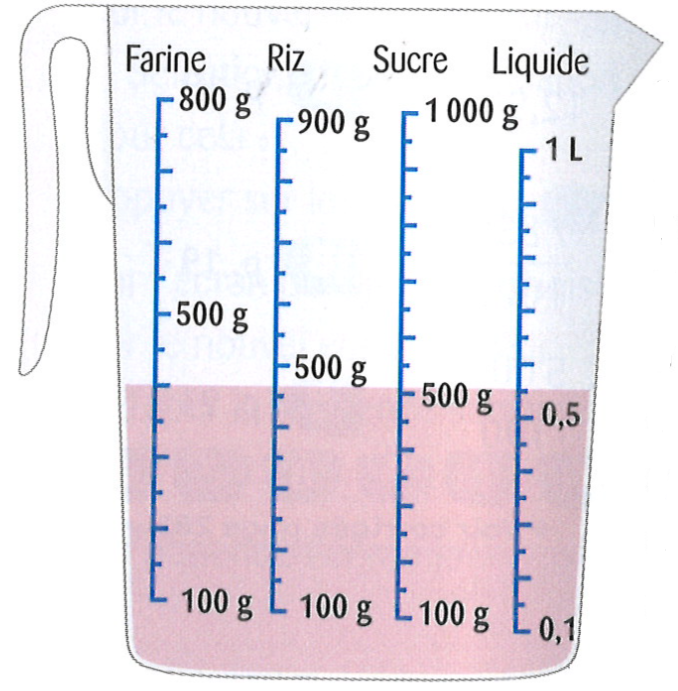
\includegraphics[scale=0.9]{img/verre}
\end{center}
\begin{questions}
	
	\begin{multicols}{4}
		
	\question[] \ 
	
	de farine ? 
	
	
	\question[] \ 
	
	de riz ?
	
	
	\question[] \ 
	
	de sucre ? 
	
	
	\question[] \ 
	
	d'huile ?
	\end{multicols}
	
\end{questions}